%% figs/pareto_loss_iter.tex — TikZ wireframe stub for Figure 2.
%% Cost-Quality Pareto across the eleven LLM checkpoints.
%% Populate from paper/data/extracted_logs.csv after mlcad_runner D8.

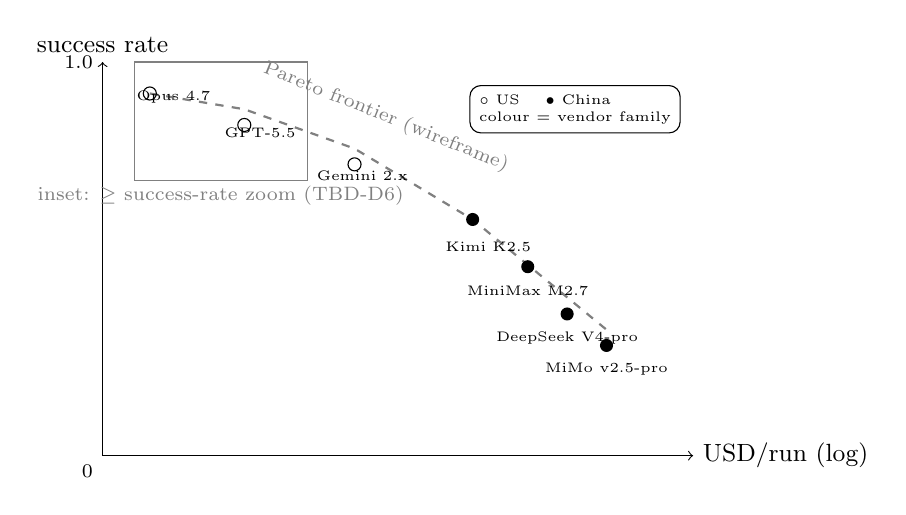
\begin{tikzpicture}
  %% Axes
  \draw[->] (0,0) -- (7.5,0) node[right] {\small USD/run (log)};
  \draw[->] (0,0) -- (0,5.0) node[above] {\small success rate};
  \node[below left] at (0,0) {\scriptsize 0};
  \node[left] at (0,5) {\scriptsize 1.0};

  %% Dashed Pareto-frontier envelope (wireframe placeholder)
  \draw[thick, dashed, gray]
    (0.6,4.6) -- (1.8,4.4) -- (3.2,3.9) -- (4.7,3.0) -- (6.4,1.6);
  \node[gray, rotate=-22] at (3.6,4.3) {\scriptsize Pareto frontier (wireframe)};

  %% Vendor-family marker legend (top-right)
  \node[draw, rounded corners, fill=white, font=\tiny, align=left]
    at (6.0,4.4) {%
      $\circ$ US \quad $\bullet$ China \\
      colour $=$ vendor family};

  %% Anchor labels for the four annotated checkpoints (wireframe)
  \node[font=\tiny] at (0.9,4.55) {Opus 4.7};
  \node[font=\tiny] at (2.0,4.10) {GPT-5.5};
  \node[font=\tiny] at (3.3,3.55) {Gemini 2.x};
  \node[font=\tiny] at (4.9,2.65) {Kimi K2.5};
  \node[font=\tiny] at (5.4,2.10) {MiniMax M2.7};
  \node[font=\tiny] at (5.9,1.50) {DeepSeek V4-pro};
  \node[font=\tiny] at (6.4,1.10) {MiMo v2.5-pro};

  %% Sample points (US = open circles, China = filled)
  \node[circle, draw, scale=0.5] at (0.6,4.6) {};
  \node[circle, draw, scale=0.5] at (1.8,4.2) {};
  \node[circle, draw, scale=0.5] at (3.2,3.7) {};
  \node[circle, fill, scale=0.5] at (4.7,3.0) {};
  \node[circle, fill, scale=0.5] at (5.4,2.4) {};
  \node[circle, fill, scale=0.5] at (5.9,1.8) {};
  \node[circle, fill, scale=0.5] at (6.4,1.4) {};

  %% Inset placeholder (high-success-rate zoom)
  \draw[thin, gray]
    (0.4,3.5) rectangle (2.6,5.0);
  \node[font=\tiny, gray] at (1.5,3.3)
    {\scriptsize inset: $\ge\tbdcell$ success-rate zoom (TBD-D6)};
\end{tikzpicture}
